\section{Collection kernels and recoil discrimination}\label{sec:20.5}

A silicon nucleus recoiling with \SI{100}{eV} makes 2.7 electron--hole pairs on average, at the measured yield $Y_q = 0.102$ and the \SI{3.8}{eV} per pair of the measurement~\cite[Eq.~(1), Table~II]{albakry2023first}; an electron recoil of the same energy makes 27. The rest of each deposit becomes phonons, and the phonon sensors see three populations: the primary phonons of the recoil, the Luke phonons of the drifting carriers, and the phonons that return the gap energy of the pairs (\cref{sec:19.5}). Charge readout separates the two recoils by the pair number, and 2.7 against 27 pairs is a separation of many standard deviations. Can a phonon readout do the same, either through the pair number, which sets the size of the Luke and gap-energy populations, or through a difference in the primary phonons themselves? Both routes depend on one object, the collection kernel of each sensor. From the kernels follows what fixes the sign of the collection ratio $\mathfrak{r}_{\mathrm{coll}} - 1$, which \cref{sec:19.5} left open, and the ceiling of a readout at high bias.

\subsection{Collection kernels}\label{sec:20.5-kernels}

Since the transport of \cref{sec:20.2,sec:20.3,sec:20.4} is linear in the birth spectrum (\cref{sec:20.2-prompt}), let a population $X \in \{\mathrm{prim}, \mathrm{Luke}, \mathrm{gap}\}$ be born at the event position $\vect{r}_{\mathrm{ev}}$ with the spectral energy density $u_X(E_{\mathrm{ath}})$ and the total energy $E_X = \int\dd E_{\mathrm{ath}}\,u_X$. Linearity then fixes the energy that sensor $s$ turns into quasiparticles as
\begin{equation}
  E_{s,X}(\vect{r}_{\mathrm{ev}}) = \int\dd E_{\mathrm{ath}}\;\mathfrak{C}_s(E_{\mathrm{ath}};\vect{r}_{\mathrm{ev}})\,u_X(E_{\mathrm{ath}}) ,
  \label{eq:20.5-kernel}
\end{equation}
where the collection kernel $\mathfrak{C}_s(E_{\mathrm{ath}};\vect{r}_{\mathrm{ev}})$ is the fraction of the energy of phonons born with energy $E_{\mathrm{ath}}$ at $\vect{r}_{\mathrm{ev}}$ that ends as quasiparticles in sensor $s$. It contains everything between birth and signal: down-conversion and isotope scattering in the substrate, transmission into the film and back with probabilities $\bar t_{12}$ and $\bar t_{\mathrm{esc}}$, pair breaking with the yield $Y_{\mathrm{qp}}$, and loss on bare faces and holders. A phonon below $2\Delta_{\mathrm{BCS}}$ of the film cannot break a pair there and returns to the crystal, and its energy stays in the kernel's bookkeeping until another surface takes it.

The kernels belong to the detector; the two recoils differ only in how much energy they put into each population and, possibly, in the spectrum of the primaries. Every readout quantity of \cref{sec:19.5} and of this section is a linear functional of the kernels. A detector with two sensor channels (two films, or the fast and slow parts of one pulse) has the channel fraction $a_X(\vect{r}_{\mathrm{ev}}) = E_{2,X}/(E_{1,X} + E_{2,X})$ for each population, where channel 2 is the one that favors soft phonons, and the efficiency $\epsilon_X = (E_{1,X} + E_{2,X})/E_X$.
\begin{keyresult}[Readout functionals of the collection kernels]
With the channel fractions $a_X$ and efficiencies $\epsilon_X$ built from \cref{eq:20.5-kernel},
\begin{gather}
  \varpi_O = \bigl\langle a_{\mathrm{Luke}} - a_{\mathrm{prim}}\bigr\rangle_{\vect{r}} , \qquad
  \varpi_{\mathrm{gap}} = \bigl\langle a_{\mathrm{gap}} - a_{\mathrm{prim}}\bigr\rangle_{\vect{r}} , \nonumber\\
  \sigma_{\mathrm{pos}}^2 = \operatorname{Var}_{\vect{r}}\bigl[a_{\mathrm{prim}}(\vect{r}_{\mathrm{ev}}) - \hat a(\hat{\vect{r}}_{\mathrm{ev}})\bigr] , \qquad
  \mathfrak{r}_{\mathrm{coll}} = \frac{\epsilon_{\mathrm{Luke}}}{\epsilon^{\mathrm{ER}}_{\mathrm{prim}}} ,
  \label{eq:20.5-functionals}
\end{gather}
where $\langle\cdot\rangle_{\vect{r}}$ and $\operatorname{Var}_{\vect{r}}$ average over the event positions of the calibration, and $\hat a(\hat{\vect{r}}_{\mathrm{ev}})$ is the channel fraction predicted from the position $\hat{\vect{r}}_{\mathrm{ev}}$ reconstructed from the pulses. The collection contrasts $\varpi_O$ and $\varpi_{\mathrm{gap}}$ say how differently a channel sees Luke and gap-energy phonons from primaries; the position spread $\sigma_{\mathrm{pos}}$ is the part of the primary channel fraction that the position correction leaves.
\end{keyresult}
\noindent A detector is therefore characterized for every population and every recoil by two kernels on the plane $(E_{\mathrm{ath}}, \vect{r}_{\mathrm{ev}})$. The collection ratio of \cref{sec:19.5} compares two populations of the same detector, so its sign depends only on how the kernels weigh soft Luke phonons against the hard primaries that arrive after down-conversion.

The kernels of a real detector are a transport calculation. A transport Monte Carlo follows phonons launched as monochromatic sources on a grid of energies and positions, which is what turns the tallies into kernels, and \cref{app:E.25} specifies the grids, the two geometries, the acceptance tests and the pitfalls. Two of the pitfalls decide the result. Luke birth spectra must come from the carrier transport at each field, and the fate of phonons below $2\Delta_{\mathrm{BCS}}$ must be stated with every result. No kernel of a real detector has been computed, and transport codes are not yet validated against the relations of this chapter (\cref{sec:20.1-open}).

\subsection{Mean-field kernels}\label{sec:20.5-meanfield}

One limit reduces the kernels to a linear equation in energy alone. If phonons cross the crystal many times before a surface absorbs them, the population forgets where it was born, and the kernels lose their dependence on $\vect{r}_{\mathrm{ev}}$. This holds when the diffusion time across the crystal is short compared with the absorption time, and when the faces scatter diffusely, so that every phonon of energy $E_{\mathrm{ath}}$ hits them at the same rate. In a slab of thickness $d$ an isotropic phonon with speed $v$ hits one of the two faces at the rate $v/2d$, since the mean of $|v_z|$ is $v/2$. Let a fraction $c_s$ of the face area carry film $s$, with transmission $\bar t$ into it and pair-breaking threshold $2\Delta_s$, and let a phonon that hits a bare face be lost with probability $\ell_{\mathrm{bare}}$. The absorption rate per phonon is then
\begin{equation}
  \varGamma_{\mathrm{abs}}(E_{\mathrm{ath}}) = \frac{\bar v}{2d}\Bigl[\sum_s c_s\,\bar t\,\Theta(E_{\mathrm{ath}} - 2\Delta_s) + \Bigl(1 - \sum_s c_s\Bigr)\ell_{\mathrm{bare}}\Bigr] ,
  \label{eq:20.5-Gabs}
\end{equation}
with $\bar v$ the number-weighted mean speed of the mixed population and $\Theta$ the step function. Down-conversion acts at the mean rate $f_{\mathrm{LA}}\varGamma_{\mathrm{anh}}(E_{\mathrm{ath}})$ of \cref{sec:20.2-scaling}, since only longitudinal phonons decay and isotope scattering keeps their share at $f_{\mathrm{LA}}$, and a decay at $E'$ passes the energy fraction $y$ to its daughters with the energy-weighted distribution $P_{\mathrm{d}}(y)$ of \cref{eq:20.2-frag}. The number of daughters in $\dd E$ is then $P_{\mathrm{d}}(E/E')\,\dd E/E$, and the time-integrated number spectrum $\mathcal{N}(E_{\mathrm{ath}})$ of a population with birth number spectrum $n_0$ obeys
\begin{equation}
  \bigl[\varGamma_{\mathrm{abs}}(E) + f_{\mathrm{LA}}\varGamma_{\mathrm{anh}}(E)\bigr]\mathcal{N}(E) = n_0(E) + \int_E^\infty\frac{\dd E'}{E}\,P_{\mathrm{d}}\Bigl(\frac{E}{E'}\Bigr)f_{\mathrm{LA}}\varGamma_{\mathrm{anh}}(E')\,\mathcal{N}(E') ,
  \label{eq:20.5-meanfield}
\end{equation}
with $E \equiv E_{\mathrm{ath}}$. Integrating the time-dependent equation for the number spectrum from zero to infinity gives \cref{eq:20.5-meanfield}, since every phonon is eventually absorbed or lost. The equation is triangular, because daughters are softer than their parent, and it is solved from the top energy down. Sensor $s$ receives $\int\dd E\,E\,\varGamma_s(E)\mathcal{N}(E)\,Y_{\mathrm{qp},s}(E)$, where $\varGamma_s$ is its term in \cref{eq:20.5-Gabs}. The mean-field kernel is this quantity for a monochromatic source, divided by its energy.

For an estimate we take a silicon slab \SI{4}{mm} thick, the thickness of a gram-scale detector with an eV-scale threshold~\cite[Sect.~IV]{ren2021design}. The isotropic sound speeds $c_{\mathrm{LA}} = \SI{9.00}{km/s}$ and $c_{\mathrm{T}} = \SI{5.40}{km/s}$ of \cref{app:C.18} give $\bar v = \SI{5.75}{km/s}$; we take $f_{\mathrm{LA}} = 0.093$ and $A_{\mathrm{anh}} = \SI{7.41e-56}{s^4}$, the silicon values of \cref{sec:20.2}, and the stand-in $P_{\mathrm{d}}(y) = 60\,y^3(1 - y)^2$. Two films cover \SI{5}{\percent} of the face area each: one with the niobium-like threshold $2\Delta_s = \SI{3.0}{meV}$, one of aluminum with \SI{0.36}{meV}. We take $\bar t = 0.9$, close to the acoustic-mismatch average 0.938 for silicon into aluminum (\cref{sec:20.3}), and $\ell_{\mathrm{bare}} = 10^{-3}$, the loss per surface bounce measured in CDMS detectors~\cite[Sect.~III\,G]{leman2012invited}. The film yield is the Kaplan cascade of \cref{sec:20.4} in units of each film's gap, run to $120\Delta_s$ and held there above, which affects \SI{0.1}{\percent} of the primary energy in aluminum. In a film from which phonons escape, with the ratio $t_l/t_0$ of \cref{sec:20.3}, $\bar t$ is multiplied by the probability $p_{\mathrm{pb}}$ of \cref{eq:20.4-ppb} that an entering phonon breaks a pair before it leaves, and the yield is that of \cref{fig:20-yield}. A phonon that escapes unbroken re-enters the crystal unchanged, and so do the phonons a film emits after its first pair break, its relaxation phonons and the hot phonons that escape: they return to the crystal with the spectrum the cascade gives them and can be absorbed again, so that energy is conserved. Only returned phonons below $2\Delta_{\mathrm{BCS}}$ of aluminum, which no film absorbs, end on the bare faces. The primaries are born at the top of the acoustic band, \SI{62}{meV}, since their spectrum is forgotten long before they are absorbed (\cref{sec:20.2}).

The primaries come out nearly balanced between the two films. They are absorbed within \SI{15}{\micro s}, by then down-converted to a mean energy of \SI{5.0}{meV} weighted by the absorbed energy (\SI{4.0}{meV} weighted by number), and on first absorption the niobium-like film takes \SI{40.7}{\percent} of their energy, aluminum \SI{58.2}{\percent}, and the bare faces \SI{1.2}{\percent}. Aluminum gets more because \SI{18}{\percent} of the absorbed energy arrives below \SI{3}{meV}, where only aluminum absorbs. The middle \SI{80}{\percent} of it arrives between 2.45 and \SI{7.88}{meV}, the band of \cref{fig:20-yield}(a). The relaxation phonons of the niobium-like film lie below its \SI{3}{meV} threshold but mostly above that of aluminum, and the aluminum film collects them on their return. In thick films the primaries therefore have the channel fraction $a_{\mathrm{prim}} = 0.610$ and the efficiency $\epsilon_{\mathrm{prim}} = 0.684$; deleting those phonons, as a lumped film does, would give 0.563 and 0.610.

The Luke phonons are softer, and their spectrum is the open input. For a carrier at one speed, \cref{sec:20.1-luke} gives an emitted energy weighted as $E_{\mathrm{ath}}^3$ up to $E_{\mathrm{L}}^{\max} = \frac43\langle E_{\mathrm{L}}\rangle$, so that the fraction $(x/E_{\mathrm{L}}^{\max})^4$ of it lies below any $x$. A transport Monte Carlo gives $\langle E_{\mathrm{L}}\rangle = \SI{0.84}{meV}$ for silicon electrons at \SI{1}{V/cm}, and 0.84 to \SI{4.6}{meV} over 1 to \SI{100}{V/cm}. We scan 0.75 to \SI{4.7}{meV}, a range that also covers germanium electrons at low field. Real carriers do not drift at one speed: they accelerate in the field, emit, and accelerate again, and transverse phonons, which the one-branch rate leaves out, are emitted softer. Both put more energy at low $E_{\mathrm{ath}}$. We therefore use two shapes, labeled by $\langle E_{\mathrm{L}}\rangle$: the one-speed spectrum, and a flat number spectrum up to $2\langle E_{\mathrm{L}}\rangle$ for a spread of speeds, which puts the fraction $(x/2\langle E_{\mathrm{L}}\rangle)^2$ of the energy below $x$. Which shape and which mean a drifting carrier produces at a given field is still open (\cref{sec:20.1-open}). As a reference, in the strong near-surface fields of germanium detectors the Luke phonons have about \SI{300}{GHz} for electrons and \SI{700}{GHz} for holes~\cite[Sect.~1]{hertel2012phonon}, 1.2 and \SI{2.9}{meV}, and in the low bulk field they are softer.

\begin{figure}[tbp]
  \centering
  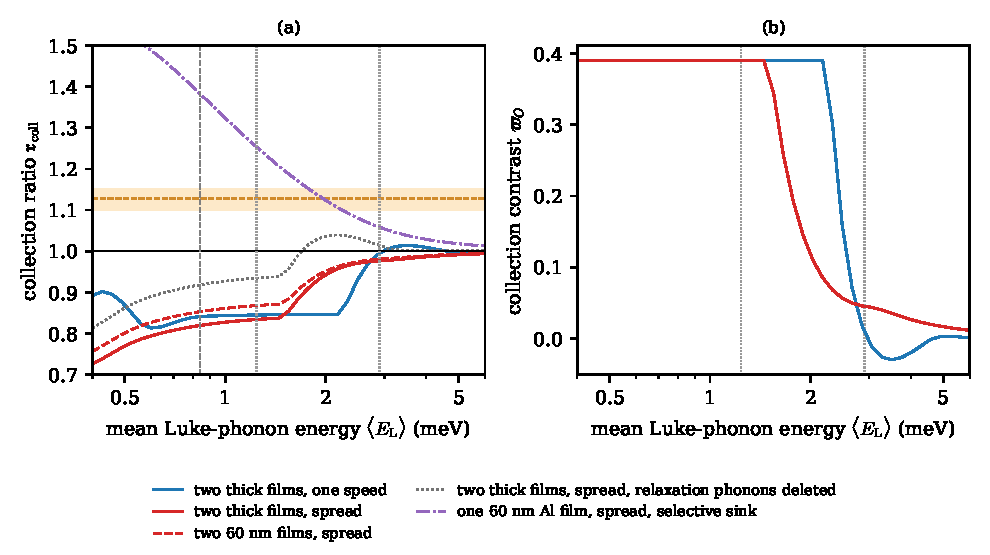
\includegraphics[width=\linewidth]{figures/ch20/fig20_rcoll.pdf}
  \caption{Mean-field collection of Luke phonons in a silicon slab \SI{4}{mm} thick, against the mean Luke-phonon energy. (a) Collection ratio $\mathfrak{r}_{\mathrm{coll}}$ of \cref{eq:20.5-functionals}. Solid: two thick films ($2\Delta_s = 3.0$ and \SI{0.36}{meV}, each on \SI{5}{\percent} of the face area) with the Kaplan-cascade yield of \cref{sec:20.4}, every phonon a film emits returned to the crystal, for the Luke spectrum of a carrier at one speed (blue, number density $\propto E_{\mathrm{ath}}^2$) and for a spread of speeds (red, flat number density up to $2\langle E_{\mathrm{L}}\rangle$). Red dashed: two \SI{60}{nm} films ($t_l/t_0 = 0.72$), spread, phonons returned. Gray dotted: two thick films, spread, with the phonons a film emits after its first pair break deleted. Purple dash-dotted: one \SI{60}{nm} aluminum film on \SI{10}{\percent} of the face area, spread, with the same deletion, a selective sink that the model does not identify in a detector (upper envelope). In all curves phonons below $2\Delta_{\mathrm{BCS}} = \SI{0.36}{meV}$ are reflected by the films and eventually lost. Tan band and dashed line: 1.099 to 1.152 and 1.128, the collection ratio that explains the silicon phonon-yield ratio of \cref{sec:19.5} with no stored energy. Vertical dashed line: \SI{0.84}{meV}, silicon electrons at \SI{1}{V/cm}; dotted: 1.24 and \SI{2.9}{meV}, the near-surface Luke energies of germanium~\cite{hertel2012phonon}. (b) Collection contrast $\varpi_O$ of the two thick films with phonons returned (channel 2 is the aluminum film), same colors. Model: transmission 0.9 into each film, bare-face loss $10^{-3}$ per hit, $\bar v = \SI{5.75}{km/s}$, $f_{\mathrm{LA}} = 0.093$, $A_{\mathrm{anh}} = \SI{7.41e-56}{s^4}$, $P_{\mathrm{d}}(y) = 60\,y^3(1 - y)^2$; primaries born at \SI{62}{meV}, absorbed in the two thick films with $\epsilon_{\mathrm{prim}} = 0.684$, $a_{\mathrm{prim}} = 0.610$.}
  \label{fig:20-rcoll}
\end{figure}

\Cref{fig:20-rcoll}(b) shows the contrast this geometry gives. While the whole Luke spectrum lies below the \SI{3}{meV} threshold of the niobium-like film, only aluminum absorbs Luke phonons, $a_{\mathrm{Luke}} = 1$, and $\varpi_O = 1 - a_{\mathrm{prim}} = 0.39$. As the mean energy rises, the Luke spectrum reaches above \SI{3}{meV} and the contrast falls: for the spread of speeds it is 0.12 at \SI{2}{meV}, 0.045 at \SI{2.9}{meV} and 0.019 at \SI{4.7}{meV}. In the mean-field limit the position spread vanishes by construction, so it is the first number a computed kernel adds.

\subsection{The sign of the collection ratio}\label{sec:20.5-sign}

The collection ratio differs from one through the part of the Luke spectrum within a few gaps of the aluminum threshold, since the primaries arrive at several meV. Luke energy below $2\Delta_{\mathrm{BCS}}$ of aluminum breaks no pairs; it is lost unless a tungsten sensor or another film absorbs it. Luke energy between $2\Delta_{\mathrm{BCS}}$ and $4\Delta_{\mathrm{BCS}}$ is converted with $Y_{\mathrm{qp}} = 2\Delta_{\mathrm{BCS}}/E_{\mathrm{ath}}$ in every film, above 0.59 below \SI{0.61}{meV} and down to 0.5 at $4\Delta_{\mathrm{BCS}}$ (\cref{sec:20.4}). Above four gaps a thick film converts with 0.59 to 0.60; a film from which phonons escape converts the primaries, at 14 to $44\,\Delta_{\mathrm{BCS}}$, with less than the soft Luke phonons on first absorption, but the phonons it lets out return to the crystal. And a phonon that only one film absorbs bounces longer before it is absorbed, and loses more on the bare faces.

The first two effects act alone in a detector with a single film type. Let $s_{\mathrm{sub}}$ be the share of Luke energy born below $2\Delta_{\mathrm{BCS}}$. Let sub-gap phonons be absorbed at the same rate as the others and converted with the weight $\kappa_{\mathrm{sub}}\bar Y_{\mathrm{prim}}$, where $\bar Y_{\mathrm{prim}}$ is the mean yield of the primaries as they are absorbed, and $\kappa_{\mathrm{sub}} = 0$ if they are lost and 1 if they are absorbed like hard phonons. Define the near-gap gain
\begin{equation*}
  s_{\mathrm{ng}} = \frac{1}{E_{\mathrm{Luke}}}\int_{2\Delta_{\mathrm{BCS}}}^\infty\dd E_{\mathrm{ath}}\;u_{\mathrm{Luke}}(E_{\mathrm{ath}})\Bigl[\frac{Y_{\mathrm{qp}}(E_{\mathrm{ath}})}{\bar Y_{\mathrm{prim}}} - 1\Bigr] .
\end{equation*}
If every phonon above the threshold reaches the film with the same probability per bounce, whatever its energy, the absorbed fraction is common to both populations and cancels in the ratio. The primaries are converted with $\bar Y_{\mathrm{prim}}$, the Luke phonons with $Y_{\mathrm{qp}}(E_{\mathrm{ath}})$ above the threshold and with $\kappa_{\mathrm{sub}}\bar Y_{\mathrm{prim}}$ below it, and
\begin{equation}
  \mathfrak{r}_{\mathrm{coll}} - 1 = s_{\mathrm{ng}} - (1 - \kappa_{\mathrm{sub}})\,s_{\mathrm{sub}} \qquad \text{(one film type)} .
  \label{eq:20.5-sign}
\end{equation}

The sub-gap share is fixed by the Luke spectrum alone. For the one-speed spectrum it is $s_{\mathrm{sub}} = 0.085$ at $\langle E_{\mathrm{L}}\rangle = \SI{0.5}{meV}$, 0.017 at \SI{0.75}{meV}, 0.011 at \SI{0.84}{meV} and $5\times10^{-3}$ at \SI{1}{meV}; for the spread of speeds 0.13, 0.058, 0.046 and 0.032, and still 0.008 at \SI{2}{meV}. In a thick film $\bar Y_{\mathrm{prim}} = 0.590$, and the near-gap gain is small: $+0.002$ for the one-speed spectrum and $+0.018$ for the spread of speeds at \SI{0.75}{meV}, since the cascade yield lies above 0.59 between 5 and $8\Delta_{\mathrm{BCS}}$ and below it near $4\Delta_{\mathrm{BCS}}$. With sub-gap phonons lost, one thick aluminum film then has $\mathfrak{r}_{\mathrm{coll}} = 0.985$ and 0.960 at \SI{0.75}{meV} and 0.994 and 0.968 at \SI{0.84}{meV}, below one by about $s_{\mathrm{sub}}$. If the sensor absorbs the sub-gap phonons, that term vanishes, and $\mathfrak{r}_{\mathrm{coll}} = 1.002$ to 1.018 between 0.75 and \SI{1}{meV}.

Escape does not change this when the phonons a film lets out return to the crystal. A returned phonon reaches a film again and continues the same cascade, so escape followed by return only delays it. For one aluminum film the solve gives the thick-film values within 0.002 at every $t_l/t_0$ down to the \SI{60}{nm} of \cref{we:20-escape}, 0.995 and 0.969 at \SI{0.84}{meV}. This is a numerical result, not an identity: bare-face loss and decay on the return path break it, and it holds at the bare-face loss of $10^{-3}$. A sink without signal that takes every phonon, modeled by raising the bare-face loss to 0.3 per hit, lowers $\epsilon_{\mathrm{prim}}$ to 0.08 and moves $\mathfrak{r}_{\mathrm{coll}}$ of the \SI{60}{nm} film only to 1.023 and 0.988. A large rise needs a selective sink, one that removes the phonons a film emits after its first pair break and leaves those that have not yet entered a film. The lumped film of \cref{sec:20.4} makes exactly that assumption. With it, the primaries are read at the yield of the band, about 0.50 at $t_l/t_0 = 4$ and 0.32 at 0.72, while the soft Luke energy keeps $2\Delta_{\mathrm{BCS}}/E_{\mathrm{ath}}$; the near-gap gain at \SI{0.75}{meV} becomes $+0.13$ and $+0.11$ at $t_l/t_0 = 4$ and $+0.61$ and $+0.49$ at 0.72, and one aluminum film at \SI{0.84}{meV} reaches 1.05 to 1.10 at $t_l/t_0 = 4$, about \SI{300}{nm}, and 1.30 to 1.53 at \SI{60}{nm}. These values are an upper envelope of the lumped-film assumption; the estimate does not identify a physical sink in a detector that would realize it.

The two-film geometry adds the third effect. Luke phonons below \SI{3}{meV} reach only the aluminum film, so they stay \SI{30}{\micro s} in the crystal against \SI{15}{\micro s} for phonons that both films absorb, and they lose twice as much on the bare faces, \SI{2.0}{\percent} against \SI{1.0}{\percent}. With a flat yield of 0.59 above each threshold and sub-gap phonons absorbed by the aluminum sensor, this alone gives $\mathfrak{r}_{\mathrm{coll}} = 0.992$, and with sub-gap phonons lost 0.935 at \SI{0.75}{meV} to 0.998 at \SI{4.7}{meV} for the spread of speeds. The film cascade with its returned phonons lowers these values further. The primaries reach the niobium-like film in large part, and its relaxation phonons, below \SI{3}{meV}, return and are collected by the aluminum film, which raises $\epsilon_{\mathrm{prim}}$ to 0.684; Luke phonons below \SI{3}{meV} gain nothing of the kind. Two thick films then give 0.83 and 0.81 at \SI{0.75}{meV} (one speed and spread), 0.84 and 0.82 at \SI{0.84}{meV}, and rise to 1.01 near \SI{3.5}{meV} for one speed, once the Luke spectrum itself reaches the niobium-like threshold. Two \SI{60}{nm} films give 0.85 to 1.01 over 0.75 to \SI{4.7}{meV}.

With every phonon a film emits returned to the crystal and energy conserved, the mean-field estimate lies between 0.81 and 1.02 over 0.75 to \SI{4.7}{meV}, one or two films, any film thickness from \SI{60}{nm} up, sub-gap phonons lost or absorbed, and between 0.82 and 1.01 at the \SI{0.84}{meV} of silicon electrons at \SI{1}{V/cm}. A signal-free sink acting on all phonons keeps it below 1.03. The collection ratio 1.128, with its band 1.099 to 1.152, that would explain the CDMS~II silicon phonon-yield ratio with no stored energy (\cref{sec:19.5}) therefore lies above the transport estimate; only the selective sink of the lumped film reaches it. Only computed kernels for real detector geometries can exclude collection as the whole explanation, and the two-bias measurement of \cref{sec:19.5} decides between collection and stored energy.

\subsection{Phonon signatures of the recoil type}\label{sec:20.5-routes}

A phonon readout separates the two recoils through an observable $O_{\mathrm{obs}}$ of each event, such as the channel fraction $E_2/(E_1 + E_2)$ or the share of the pulse in a fast window. At equal total phonon energy, the separation
\begin{equation}
  \mathcal{S}_{\mathrm{sep}} = \frac{\bigl|\langle O_{\mathrm{obs}}\rangle_{\mathrm{NR}} - \langle O_{\mathrm{obs}}\rangle_{\mathrm{ER}}\bigr|}{\bigl[\tfrac12\bigl(\sigma_{\mathrm{NR}}^2 + \sigma_{\mathrm{ER}}^2\bigr)\bigr]^{1/2}} ,
  \label{eq:20.5-sep}
\end{equation}
measures the distance between the two distributions in units of their spreads, and we call a route useful where $\mathcal{S}_{\mathrm{sep}} \ge 2$. For two Gaussians of equal width cut at the midpoint, $\mathcal{S}_{\mathrm{sep}} = 2$ accepts \SI{84}{\percent} of one population and rejects \SI{84}{\percent} of the other, and a leakage of $10^{-3}$ needs $\mathcal{S}_{\mathrm{sep}} = 6.2$, so ``useful'' is far from background-free. Let $\varphi_X$ be the share of population $X$ in the signal. Since the shares sum to one, the channel fraction is $O_{\mathrm{obs}} = \sum_Xa_X\varphi_X = a_{\mathrm{prim}} + \varpi_O\,\varphi_{\mathrm{Luke}} + \varpi_{\mathrm{gap}}\,\varphi_{\mathrm{gap}}$ after the average over positions, and another observable linear in the delivered energies has the same form to first order in the contrasts. There is one route for each population.

\paragraph{Primary phonons.} The prompt phonons forget their polarization within a nanosecond, and a hard birth once $E_*(t)$ has fallen to about half its energy (\cref{sec:20.2-memory}). The soft energy remains. It is the share $f_{\mathrm{s}} = \SI{1.7}{\percent}$ of an electron recoil that its carriers shed below the optical phonon energy, \cref{eq:20.2-fs}. A nuclear recoil has $Y_q$ times as many pairs, and its lattice share is born near the optical and zone-boundary energies (\cref{sec:19.1}). If $E_{\mathrm{mem}}$ lies above the soft band and below every hard birth, \cref{eq:20.2-bound} then gives
\begin{equation}
  \bigl|\langle O_{\mathrm{obs}}\rangle_{\mathrm{NR}} - \langle O_{\mathrm{obs}}\rangle_{\mathrm{ER}}\bigr| \simeq \varpi_{\mathrm{soft}}\,\Delta_{\mathrm{soft}} , \qquad \Delta_{\mathrm{soft}} = (1 - Y_q)\,f_{\mathrm{s}} ,
  \label{eq:20.5-primary}
\end{equation}
with $\varpi_{\mathrm{soft}}$ the contrast of the channel between soft primaries and hard ones. This is an estimate, not a bound (\cref{sec:20.2-bound}). At \SI{100}{eV}, $\Delta_{\mathrm{soft}} = 0.015$. The spread includes the position spread, so $\mathcal{S}_{\mathrm{sep}} \le \varpi_{\mathrm{soft}}\Delta_{\mathrm{soft}}/\sigma_{\mathrm{pos}}$, and any $\sigma_{\mathrm{pos}}$ above $\Delta_{\mathrm{soft}}/2 = 0.008$ excludes a useful separation at every energy, even with a perfect selector, $\varpi_{\mathrm{soft}} = 1$. The selector is far from perfect: the soft births have a few meV, and the mean-field estimate of \cref{sec:20.5-meanfield} puts the energy of the hard primaries at a mean of \SI{5.0}{meV} when they are absorbed, so no film threshold separates the two bands. The pulse shapes of CDMS detectors depend strongly on how close the event lies to each instrumented face~\cite[Sect.~2]{hertel2012phonon}, and a position correction must reach the percent level before this route opens. Phonons born within the memory-loss distance of an instrumented face keep some memory, but they mark a position class, not a recoil type (\cref{sec:20.2-memory}). None of this holds for sapphire, where isotope mixing is slower than decay and the memory argument of \cref{sec:20.2} fails.

\paragraph{Gap energy at zero field.} Each pair carries $\Eg$ until it recombines, so an electron recoil holds $\Eg/\varepsilon_{\mathrm{eh}} = 0.312$ of its energy in pairs, a nuclear recoil $Y_q$ times as much (\cref{sec:19.5}). If this energy comes back later than the primaries, a sensor with two read windows $t_1 < t_2$, with all gap energy returned by $t_2$, sees the ratio $O_b = E_{\mathrm{sig}}(t_1)/E_{\mathrm{sig}}(t_2)$. With $f_{\mathrm{ret}}(t)$ the returned fraction of \cref{eq:19.5-release}, no stored energy and equal collection,
\begin{equation}
  \Delta O_b = \frac{\Eg}{\varepsilon_{\mathrm{eh}}}\Bigl\{\bigl[1 - f^{\mathrm{ER}}_{\mathrm{ret}}(t_1)\bigr] - Y_q\bigl[1 - f^{\mathrm{NR}}_{\mathrm{ret}}(t_1)\bigr]\Bigr\} .
  \label{eq:20.5-gap}
\end{equation}
For equal release laws this is $(1 - Y_q)(\Eg/\varepsilon_{\mathrm{eh}})(1 - f_{\mathrm{ret}}) = 0.28\,(1 - f_{\mathrm{ret}})$ at \SI{100}{eV}, twenty times the primary estimate. The route is a timing reading of the pair number, and its size and sign are set by kinetics that are not known at millikelvin. In the dense track of a nuclear recoil, exciton annihilation gives $1 - f^{\mathrm{NR}}_{\mathrm{ret}} = 1/(1 + t/t_{\mathrm{rel}})$, with $t_{\mathrm{rel}}$ the time scale set by the initial track density (\cref{eq:19.5-bimol}). Against an exponential release $\ee^{-t/t_{\mathrm{rel}}}$ of the electron recoil on the same time scale, $\Delta O_b$ changes sign at the root of $\ee^{-x}(1 + x) = Y_q$, which is $t_1 = 3.87\,t_{\mathrm{rel}}$ at $Y_q = 0.102$. The site matters as much as the time. Release in the bulk produces hard phonons that lose their memory, and contributes nothing to $\varpi_{\mathrm{gap}}$. Release at a surface or an electrode produces soft phonons that travel ballistically, like the recombination phonons that carry \SI{13}{\percent} of the phonon signal of germanium detectors at \SI{3}{V} (\cref{sec:20.4-electrode}). The zero-field gap-energy channel is therefore unresolved.

\paragraph{Luke phonons at low bias.} With a bias the Luke share differs between the recoils because the pair number does. Let all pairs be drifted, with $g = f_{\mathrm{det}}\,g_{\mathrm{Luke}}$. An electron recoil then has $\varphi_{\mathrm{Luke}} = g/(1 + g)$ and a nuclear recoil $Y_qg/(1 + Y_qg)$. The gap shares differ in the same way, so
\begin{equation}
  \Delta O_{\mathrm{obs}} = \frac{(1 - Y_q)\,\bigl(\varpi_O\,g + \varpi_{\mathrm{gap}}\Eg/\varepsilon_{\mathrm{eh}}\bigr)}{(1 + g)(1 + Y_qg)} .
  \label{eq:20.5-lowbias}
\end{equation}
The Luke term is largest at $g = Y_q^{-1/2}$, where it equals $\varpi_O(1 - Y_q^{1/2})/(1 + Y_q^{1/2})$: at \SI{100}{eV}, $0.516\,\varpi_O$ at $g = 3.1$, or \SI{13.4}{V} across a silicon crystal at $f_{\mathrm{det}} = 0.873$. Whether the contrast suffices depends on the spreads. We compare the two recoils at the same recoil energy, \SI{100}{eV}, with the pair numbers of the measured yield in pairs of $\varepsilon_{\mathrm{eh}}$, $Y'_q$ of \cref{sec:20.5-hv}. The spread of $O_{\mathrm{obs}}$ for each recoil is the position spread, the baseline $\sigma_{\mathrm{ph}} = \SI{2.65}{eV}$ of the gram-scale detector~\cite{ren2021design} divided by that recoil's $E_{\mathrm{ph}}$, and the fluctuation of its detected pair number, $\varpi_O(eV_{\mathrm{bias}}/E_{\mathrm{ph}})(F_{\mathrm{meas}}N_{\mathrm{det}})^{1/2}$, added in quadrature. The binomial form of the measured-charge Fano factor, $F_{\mathrm{meas}} = f_{\mathrm{det}}F + 1 - f_{\mathrm{det}}$ (\cref{sec:20.1-fano}), uses the measured $F_{\mathrm{eh}} = 0.119$ for electron recoils, the measured $F_{\mathrm{NR}} = 0.9$ at \SI{100}{eV}~\cite[Table~II]{albakry2023first}, and $f_{\mathrm{det}} = 0.873$, the complement of the \SI{12.7}{\percent} trapping probability in the detector model of the same measurement. With $\varpi_{\mathrm{gap}} = 0$, the smallest contrast that reaches $\mathcal{S}_{\mathrm{sep}} = 2$ at \SI{100}{eV} is $\varpi_O = 0.11$, 0.22 and 0.43 for $\sigma_{\mathrm{pos}} = 0.02$, 0.05 and 0.10, at biases of 10 to \SI{12}{V}. The mean-field contrast of about 0.4 for Luke spectra below \SI{1.5}{meV} is within reach of this requirement, but it is a model, not a measurement. The route reads the pair number with phonons. Its ceiling, with $\varpi_O = 1$ and no other spread, is reached as the bias goes to zero, and it is that of the charge yield itself, 10.8 at \SI{100}{eV}: the route carries no information beyond the charge yield.

The phonon pulse-shape rejection of SuperCDMS germanium detectors is of this kind. It rejects bulk electron recoils against nuclear recoils at better than 1 in $10^3$ at 7 to \SI{20}{keV}, limited by the statistics of the data~\cite[Sect.~3]{hertel2012phonon}, and its information comes from Luke phonons emitted in the strong field near the surfaces.

\subsection{The high-voltage readout ceiling}\label{sec:20.5-hv}

At \SI{100}{V} across a silicon crystal, $g_{\mathrm{Luke}} = 26.7$ and the Luke phonons dominate the signal. Detectors run this way read the pair number through the total phonon energy, $E_{\mathrm{ph}} = E_{\mathrm{prim}} + N_{\mathrm{det}}eV_{\mathrm{bias}}$ with $N_{\mathrm{det}}$ the detected pairs (\cref{sec:1.5}), and an electron recoil of the same $E_{\mathrm{ph}}$ is the background to a nuclear recoil. Suppose a second observable reads the Luke share perfectly, with $\varpi_O = 1$, no baseline noise and no position spread. Its separation is the most any phonon observable can extract from the pair number at high bias.

A nuclear recoil of energy $E_R$ makes on average $Y_qE_R/\varepsilon_{\mathrm{src}}$ pairs, where $\varepsilon_{\mathrm{src}} = \SI{3.8}{eV}$ is the energy per pair with which the measurement converted its charge into the yields~\cite[Eq.~(1)]{albakry2023first}; write $Y'_q = Y_q\varepsilon_{\mathrm{eh}}/\varepsilon_{\mathrm{src}}$, so that the pair number is $Y'_qE_R/\varepsilon_{\mathrm{eh}}$. Its phonon energy is $E_{\mathrm{ph}} = E_R(1 + gY'_q)$, with $g = f_{\mathrm{det}}g_{\mathrm{Luke}}$ and the primary phonon energy taken equal to the recoil energy, the truncation of \cref{lim:19.5a} that the measurement uses. The electron recoil with the same $E_{\mathrm{ph}}$ has the energy $E_R(1 + gY'_q)/(1 + g)$. Their mean detected pair numbers are
\begin{equation*}
  \langle N_{\mathrm{det}}\rangle_{\mathrm{NR}} = f_{\mathrm{det}}Y'_q\frac{E_R}{\varepsilon_{\mathrm{eh}}} , \qquad
  \langle N_{\mathrm{det}}\rangle_{\mathrm{ER}} = f_{\mathrm{det}}\frac{E_R}{\varepsilon_{\mathrm{eh}}}\,\frac{1 + gY'_q}{1 + g} ,
\end{equation*}
and their difference is $f_{\mathrm{det}}(E_R/\varepsilon_{\mathrm{eh}})(1 - Y'_q)/(1 + g)$. The Luke share at fixed $E_{\mathrm{ph}}$ is linear in $N_{\mathrm{det}}$, so its separation is that of $N_{\mathrm{det}}$, with variances $F^X_{\mathrm{eff}}\langle N_{\mathrm{det}}\rangle_X$.
\begin{keyresult}[High-voltage readout ceiling]
With an ideal readout of the Luke share at equal total phonon energy, the separation of nuclear from electron recoils is
\begin{equation}
  \mathcal{S}_{\mathrm{HV}} = \frac{(1 - Y'_q)\,(f_{\mathrm{det}}E_R/\varepsilon_{\mathrm{eh}})^{1/2}}{\bigl\{\tfrac12(1 + g)\bigl[F^{\mathrm{NR}}_{\mathrm{eff}}\,Y'_q(1 + g) + F^{\mathrm{ER}}_{\mathrm{eff}}(1 + gY'_q)\bigr]\bigr\}^{1/2}} , \qquad g = f_{\mathrm{det}}\,g_{\mathrm{Luke}} ,
  \label{eq:20.5-hv}
\end{equation}
with $F_{\mathrm{eff}} = f_{\mathrm{det}}F + 1 - f_{\mathrm{det}}$ when a trapped carrier induces nothing and $F_{\mathrm{eff}} = f_{\mathrm{det}}F$ when every pair induces the mean charge $f_{\mathrm{det}}e$. The cascade and partial-charge terms of \cref{eq:20.1-Fpos} lie between these limits.
\end{keyresult}
\noindent At zero gain \cref{eq:20.5-hv} is the separation of an ideal charge-and-heat measurement. As the bias grows it falls as $1/g$, because at equal total phonon energy a larger Luke gain makes the electron recoil smaller, and the two pair numbers converge. In silicon at \SI{220}{eV} the ceiling is 16.8 at zero bias, 10.7 at \SI{4}{V}, 3.4 at \SI{30}{V}, 1.22 at \SI{100}{V} and 0.43 at \SI{300}{V}.

\begin{workedexample}{The high-voltage ceiling at 220 eV}\label{we:20-ceiling}
The measured silicon yield at $E_R = \SI{220}{eV}$ is $Y_q = 0.108^{+0.009}_{-0.010}$, with the pair-number Fano factor $F_{\mathrm{NR}} = 0.5^{+0.2}_{-0.1}$~\cite[Table~II]{albakry2023first}. At \SI{100}{V}, $g_{\mathrm{Luke}} = 100/3.75 = 26.67$, and with $f_{\mathrm{det}} = 0.873$, $g = 23.28$. The yield in pairs of \SI{3.75}{eV} is $Y'_q = 0.108\times3.75/3.8 = 0.1066$, and $E_R/\varepsilon_{\mathrm{eh}} = 58.67$.

The nuclear recoil has $E_{\mathrm{ph}} = 220\times(1 + 23.28\times0.1066) = \SI{765.9}{eV}$, and the electron recoil with the same phonon energy has $765.9/24.28 = \SI{31.54}{eV}$. The mean detected pair numbers are $0.873\times0.1066\times58.67 = 5.459$ and $0.873\times31.54/3.75 = 7.343$, a difference of 1.885 pairs.

With trapped carriers inducing nothing, $F^{\mathrm{NR}}_{\mathrm{eff}} = 0.873\times0.5 + 0.127 = 0.5635$ and $F^{\mathrm{ER}}_{\mathrm{eff}} = 0.873\times0.119 + 0.127 = 0.2309$. The variances are $0.5635\times5.459 = 3.076$ and $0.2309\times7.343 = 1.695$, and
\begin{equation*}
  \mathcal{S}_{\mathrm{HV}} = \frac{1.885}{[\tfrac12(3.076 + 1.695)]^{1/2}} = 1.22 .
\end{equation*}
If every pair induces the mean charge instead, the trapping term drops out of both Fano factors and $\mathcal{S}_{\mathrm{HV}} = 1.50$; with full collection, $f_{\mathrm{det}} = 1$, it is 1.32. Even an ideal phonon observable cannot separate the two recoils at \SI{220}{eV} and \SI{100}{V}.
\end{workedexample}

\begin{figure}[tbp]
  \centering
  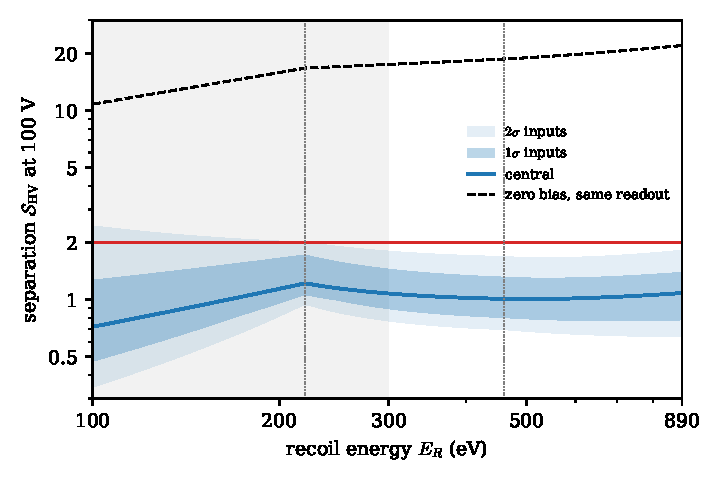
\includegraphics[width=0.8\linewidth]{figures/ch20/fig20_5.pdf}
  \caption{High-voltage readout ceiling $\mathcal{S}_{\mathrm{HV}}$ of \cref{eq:20.5-hv} for silicon recoils at \SI{100}{V}, against the recoil energy. Line: central measured yield and Fano factor~\cite[Table~II]{albakry2023first} at 100, 220, 460 and \SI{890}{eV} (dotted verticals), interpolated linearly in $\log E_R$; detected fraction $f_{\mathrm{det}} = 0.873$, trapped carriers inducing nothing; $F_{\mathrm{eh}} = 0.119$; $\varepsilon_{\mathrm{eh}} = \SI{3.75}{eV}$, yields defined with \SI{3.8}{eV} per pair. Dark band: the extremes over the corners of the $1\sigma$ bands of $Y_q$ and $F_{\mathrm{NR}}$, over $f_{\mathrm{det}} = 0.873$ and 1, and over the two limits of the induced-charge spread; light band: the same with $2\sigma$ bands. Dashed: the same ideal readout at zero bias. Red line: $\mathcal{S}_{\mathrm{HV}} = 2$. Gray: the range of the no-go statement, $E_R \le \SI{300}{eV}$.}
  \label{fig:20-ceiling}
\end{figure}

\Cref{fig:20-ceiling} extends the example over the measured range. At the central inputs the ceiling stays below 2 at every measured energy up to \SI{890}{eV}, with its maximum, 1.22, at \SI{220}{eV}; the Fano factor of nuclear recoils grows to 3.7 at \SI{890}{eV} and keeps it down. Over the $1\sigma$ bands of $Y_q$ and $F_{\mathrm{NR}}$ the largest value is 1.72, at \SI{220}{eV}, in the mean-charge limit. With $2\sigma$ bands the ceiling exceeds 2 from 100 to \SI{224}{eV}, up to 2.46 at \SI{100}{eV}, where the measured yield is least certain. The no-go of a high-voltage phonon readout at $E_R \le \SI{300}{eV}$ therefore rests on the measured $Y_q$ and $F_{\mathrm{NR}}$, which are not derived below the binary threshold of \cref{sec:19.2}, and on the collection, which moves the ceiling at \SI{220}{eV} between 1.22 and 1.50.

\subsection{Uncertainty budget of the readout}\label{sec:20.5-budget}

\Cref{tab:20-nuisances} is the uncertainty budget of the chapter.
\begin{table}[tbp]
  \caption{Uncertainty budget of charge, phonon and quasiparticle readout. Classes and bases as in \cref{tab:10-nuisances}; ``delayed'' moves charge or energy in time over an exposure.}
  \label{tab:20-nuisances}
  \centering\scriptsize\setlength{\tabcolsep}{3pt}
  \begin{tabular}{@{}>{\raggedright\arraybackslash}p{0.26\linewidth}>{\raggedright\arraybackslash}p{0.12\linewidth}>{\raggedright\arraybackslash}p{0.35\linewidth}>{\raggedright\arraybackslash}p{0.09\linewidth}>{\raggedright\arraybackslash}p{0.10\linewidth}@{}}
    \toprule
    Truncation or input & Type & Size & Basis & Section \\
    \midrule
    Exponential survival of drifting carriers & normali\-zation & collected fraction 0.632 (face), 0.736 (uniform) at $\lambda_{\mathrm{d}} = d_{\mathrm{det}}$; saturating drift velocity caps it below one & computed; model & \cref{sec:20.1} \\
    Fano factor of the measured charge & normali\-zation (width) & 0.125--0.158 at \SI{100}{eV}, \SI{95}{\percent} collection; position term $1.2\times10^{-4}\,\bar N_{\mathrm{eh}}$ & computed & \cref{sec:20.1} \\
    Space charge between flashes & delayed & \SI{1}{\percent} field change at \SI{1}{V/cm} for 6.3--$12.6\times10^4$ trapped charges per \si{cm^2} & est. & \cref{sec:20.1} \\
    Athermal emission from traps & delayed & cross-sections not computed & unsized & \cref{sec:20.1} \\
    Luke emission rate and spectrum & normali\-zation (of $\mathfrak{r}_{\mathrm{coll}}$, $\varpi_O$) & transverse emission omitted; mean energy \SI{0.84}{meV} for electrons at \SI{1}{V/cm} & model; unsized & \cref{sec:20.1,sec:20.5} \\
    Memory loss of prompt phonons & tilt & \SI{6.8}{ns} (Si), \SI{47}{ns} (Ge) near the band top; about \SI{1}{\micro s} for the \SI{22}{meV} daughters in Si; fails for sapphire & est. & \cref{sec:20.2} \\
    Interface transmission model & normali\-zation & $t_l$ differs by 1.31 between acoustic and diffuse mismatch; anisotropy: $\bar t_{\mathrm{esc}} = 0.327$--0.405 & model & \cref{sec:20.3} \\
    Quasiparticle yield above $4\Delta_{\mathrm{BCS}}$ & normali\-zation & 0.590 without escape; 0.349--0.554 at $10\Delta_{\mathrm{BCS}}$ for $t_l/t_0 = 0.5$--8; kinetic equations higher by up to 0.04 & model & \cref{sec:20.4} \\
    Soft primary share of an electron recoil & tilt & $f_{\mathrm{s}} \simeq 0.017$; $(1 - Y_q)f_{\mathrm{s}} = 0.015$ at \SI{100}{eV} & est. & \cref{sec:20.2,sec:20.5} \\
    Collection ratio of Luke phonons & normali\-zation & 0.81--1.02 (energy conserved); selective sink up to 1.53; 1.128 not reached; detector kernels not computed & model & \cref{sec:20.5} \\
    Collection contrast of Luke phonons & normali\-zation & 0.39 below about \SI{1.5}{meV}, 0.045 at \SI{2.9}{meV}; the low-bias route needs 0.11--0.43 & model & \cref{sec:20.5} \\
    Position spread of the channel fraction & normali\-zation & above 0.008 it closes the primary route & unsized & \cref{sec:20.5} \\
    Release law and site of the gap energy & tilt; delayed & two-window difference up to $0.28(1 - f_{\mathrm{ret}})$ at \SI{100}{eV}; sign not known & unsized & \cref{sec:20.5} \\
    Inputs of the high-voltage ceiling & threshold & \SI{220}{eV}, \SI{100}{V}: 1.22 (central), 1.50 (mean charge); 2.46 at \SI{100}{eV} with $2\sigma$ bands & input spread & \cref{sec:20.5} \\
    \bottomrule
  \end{tabular}
\end{table}
